% !Mode:: "TeX:UTF-8"
%%% Local Variables:
%%% mode: latex
%%% TeX-master: t
%%% End:

\chapter{面向对象的遥感影像的区间二型模糊聚类分割算法}
\label{cha:chap03}

\section{引言}
\label{sec:chap03-1}
由于遥感影像数据具有同物异谱、同谱异物等固有的不确定性,结合模糊数学理论对不确定信息刻画的优点,模糊C-均值聚类(Fuzzy c-means clustering, FCM)分割方法被广泛应用到遥感影像分析中 \cite{bezdek1984fcm}。同时,随着遥感影像空间分辨率的提高,高分影像数据具有更多的信息多样性和复杂性,遥感影像聚类方法由传统的基于像元发展为面向对象的聚类分割。本章内容从遥感影像特征信息表达和目标地物类别关系两个角度来考虑遥感影像分类中不确定性信息的表达模型


本文从影像数据本身特征信息表达和影像类别间的关系描述两个角度力图设计有效的遥感影像分类不确定性表达模型,一方面设计面向分类的影像区间值信息表达模型,以刻画遥感影像类别样本个体在一定范围内的可变性和随机性,结合合理的相异性度量定义提高类别的可分性;另一方面设计二型模糊集合来对影像模式集建模,以刻画土地覆盖类别的高阶模糊不确定性,从而提高光谱近似或混叠的不同类别的区分度和光谱异质的同类别的包容性。

\begin{figure}[!htb] % use float package if you want it here
    \centering
    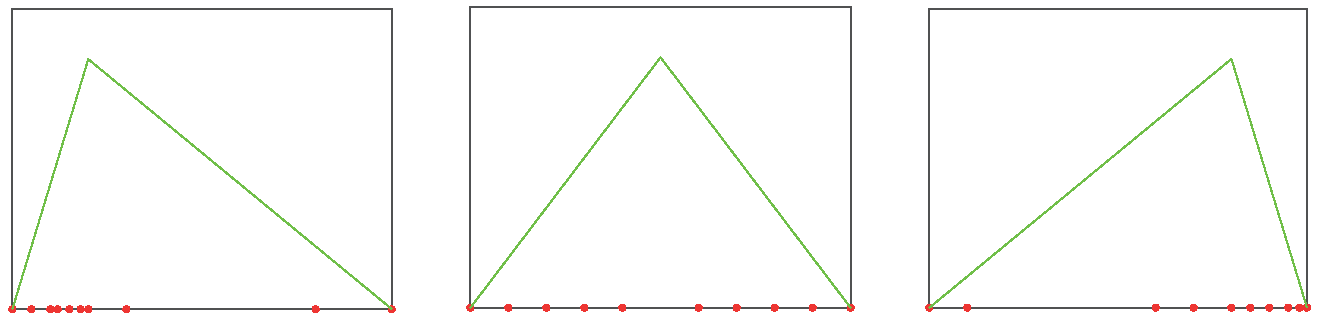
\includegraphics[width=0.8\textwidth]{compare_distribution}
    \caption{区间值相同但分布不同的数据比较}
    \label{fig:compare_distribution}
  \end{figure}

\section{三角形模糊集值的建模}
\label{sec:chap03-2}
已有的面向对象分割方法中对影像分割单元进行均值数据建模 \cite{yu2012method} 和区间值数据建模 \cite{he2016remote} 的信息表达模型无法区分具有相同均值和区间值但内部分布不一致的分割单元。如图 \ref{fig:compare_distribution} 所示,三组模拟数据内的点看作一个影像分割单元像素点集合,具有相同的
封面的例子请参看 cover.tex。主要符号表参看 denation.tex,附录和个人简历分别参看 appendix01.tex
和 resume.tex。里面的命令都非常简单,一看即会。\footnote{你说还是看不懂?怎么会呢?}

\section{字体命令}
\label{sec:first}

苏轼(1037-1101),北宋文学家、书画家。字子瞻,号东坡居士,眉州眉山(今属四川)人
